\documentclass[conference]{IEEEtran}

\usepackage{url}
\usepackage{multirow}
\usepackage{array}
\usepackage{epsfig}
\usepackage{footnote}
\usepackage{amsmath}

\widowpenalty=100000
\clubpenalty=100000

\begin{document}

\title{Grid Appliance -- On the Design of Self-Organizing,
Decentralized Grids}

\author{
\IEEEauthorblockA{
  David Isaac Wolinsky,
  Renato Figueiredo
}
\IEEEauthorblockN{
  University of Florida
}
}

\maketitle


\begin{abstract}

``Give a man a fish, feed him for a day.  Teach a man to fish, feed him for a
lifetime'' -- Lau Tzu

Grid computing projects such as TeraGrid~\cite{teragrid},
Grid'5000~\cite{grid_5000}, and OpenScience Grid~\cite{osg} enable researchers
to access vast amounts of compute resources, but in doing so, they force the
researcher to adapt their workloads to the environments these systems provide.
This does not leave many alternatives for researchers as creating these types
of systems requires coordination and expertise in networking, operating
systems, security, and grid middleware.  This results in many research groups
creating small, in-house compute clusters where scheduling is often ad-hoc (and
resource utilization is low), and aggregation of resources across multiple
groups is hindered by the complexities in constructing federated systems.  This
paper describes the ``Grid Appliance'', the first system of its kind that
enables researchers to efficiently deploy their own compute clusters, and to
seamlessly extend their systems across network domains to create small to large
scale computing grids.  The paper details the design of the Grid Appliance and
reports on experiences and lessons learned over four years of development and
deployment of wide-area Grid appliance pools.

\end{abstract}

\section{Introduction}

Grid computing presents opportunities to combine various scale, distributed
systems together to form powerful computing systems.  Due to the challenges in
coordinating the organization of grids, researchers typically become members of
existing grids or inefficiently use their own local resources, such as
coordinating with other members of the lab access to the various systems.
While there is a wealth of grid software available, most researchers see the
entry barrier to installing and management of the system as being greater than
the usefulness of the application.  Succinctly defined, the problem we address
in this paper is how to introduce complex grid middleware to users, such that
they can focus on making use of the software and not the setup and managerment
of the systems thereafter.

Our approach begins with a P2P infrastructure enabling peers to discover each
other and coordinate the organization of a grid.  We use a P2P system based
upon a distribute hash table (DHT), which enables peers to efficiently query
the system with a key and discover one or more values that map to that key.  We
also layer on top of the P2P overlay a virtual private network (VPN), which
provides all-to-all connectivity and transparently handles configuration and
organization through the DHT.  The grid middleware can use either the DHT or
the VPN to bootstrap various grid middleware stacks, such as
Condor~\cite{condor}, Torque (PBS)~\cite{torque}, Sun Grid Engine~\cite{sge},
MPICH~\cite{mpich}, or Hadoop~\cite{hadoop}.  The entire system has been
packaged into a repository to automatically configure physical, virtual, and
even cloud resources.  The resulting ``Grid Appliance'' is a preconfigured
environment emphasizing trivial installation, enabling user interaction with
the system to focus on the tools provided and not configuration details,
providing researchers with a plug-and-play tool to create ad-hoc virtual
compute clusters for their own groups, local or federated.

To justify our techniques, consider the difficulty in combining resources
across disparate networks, which may or may not involve multiple research
groups.  Challenges such as safety, security, connectivity, and efficiency
require an information technology (IT) expert.  Furthermore, network
constraints present another complexity beyond configuration and organization of
distributed resources.  An individual group may have resources behind different
network address translators (NATs) and firewalls, preventing direct
communication with each other.  Even assuming that an institution's network
administrator is willing to make exceptions for the grid, additional rules may
be required for each new cluster or resource added internally and externally,
quickly becoming unmanageable.

The grid systems considered in this paper consist of three fundamental
components:  execute nodes, resource managers, and submission nodes.  The
execute nodes run the tasks submitted from the submission sites.  Users access
a submission site, craft task description files, and submit them to a scheduler
or resource manager, which will queue tasks to the various execute nodes.

Existing work that falls under the general area of desktop grids/opportunistic
computing include Boinc~\cite{boinc}, BonjourGrid~\cite{bonjourgrid}, and
PVC~\cite{pvc}.  Boinc, used by many ``@home'' solutions, focuses on adding
execute nodes easy; however, job submission and management rely on
centralization and all tasks must use the Boinc APIs.  BonjourGrid removes the
need for centralization through the use of multicast resource discovery; the
need for which limits its applicability to local area networks.  PVC enables
distributed, wide-area systems with decentralized job submission and execution
through the use of VPNs, but relies on centralized VPN and resource management.

Each approach addresses a unique challenge in grid computing, but none
addresses the challenge presented as a whole: easily constructing distributed,
cross-domain grids.  Challenges that we consider in the design of our system
are ensuring that submission sites can exist any where and are not confined to
complex configuration or highly available, centralized locations; ability to
dynamically add and remove resources by starting and stopping an appliance; and
the ability for individual sites to share a common server or to have one or
more per site so that no group in the grid is dependent on another.  We
emphaize these points, while still retaining the ease of use of Boinc, the
connectivity of PVC, and the flexibility of BonjourGrid.  The end result is a
system similar in organization to OurGrid~\cite{ourgrid}, though with
self-configuration and organization and a VPN to transparently handle network
constraints.

``Grid Appliance'' systems can be constructed in one of two ways.  Local grids
can be constructed by booting the appliances, which will then use multicast
self-discovery to find other resources, create the DHT overlay, and then form
VPN links.  Alternatively, a wide area grid construction is managed through a
web site and bootstrapped from a P2P overlay, either our public shared
deployments or private systems easily deployed through a virtual appliance.
The web site uses a group interface, similar to online social networking
groups, as a wrapper around a certificate authority based public key
infrastructure.  Users can join a group or create their own.  To support
collaboration across groups, groups are divided into two categories: VPN groups
(used to determine nodes authorized to connect to the VPN) and institution
groups (used to determine priority in accessing resources).  In practice, each
collaborative group represents a unique VPN and each institutional group
represents a collective subset of the grid.  

\begin{figure}[h]
\centering
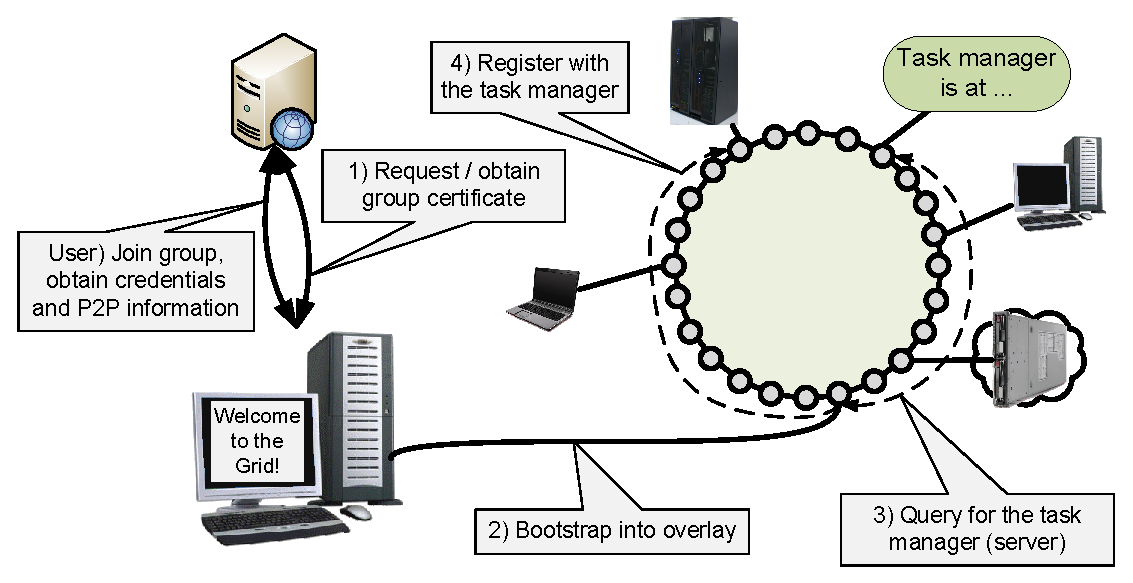
\epsfig{file=figs/system.eps, width=3.12in}
\caption{An example deployment scenario:  obtaining configuration files, to
starting the appliance, and connecting with a resource manager.}
\label{fig:system}
\end{figure}

As presented in Figure~\ref{fig:system}, users join a resource group for VPN
purposes and then an institutional group to obtain priority for resources
shared by their group.  Upon joining both groups, the user can download one of
three different types of configurations: server, worker, and client (mapping to
the three types of typical grid nodes, resource manager, execution site, and
submission site).  In addition to the configuration data, a first time user can
download the generic appliance, or one extended with additional software
customized for their community.  In the case of a virtual machine appliance,
the configuration data can be added to the system as a virtual floppy image,
automatically configuring the appliance for a specific behavior.  In the case
of the client, it begins searching for an appropriate resource manager by
querying the DHT.  Upon finding an entry in the DHT, the client communicates
with the resource manager via the VPN.  The same procedure can be repeated many
times to add additional resources into the grid.  Resources booted using the
``server'' image configure and advertise themselves through the DHT or VPN.
Each individual grid can support multiple servers for fail-over or load
balancing, depending on the capabilities of the grid middleware (e.g. Condor
flocking).  Beyond the downloading of the appliance and the configuration data,
all other steps are performed transparently from the user.

As of this date, we have focused on two uses for this system: high throughput
computing (HTC) systems for research and self-configuring modules for
education.  To this end, we have used the Condor grid middleware for our HTC,
which we will discuss shortly.  On the other spectrum, techniques that we
describe enable easy construction of educational clusters/grids, which would
otherwise be significant time sinks for students who need to learn more about
how a grid works and less about how to configure one across domains.  As of
this date, we have implemented Hadoop and MPI educational packages.  For HTC,
we chose Condor because, through simple configuration, it enables resources to
join dynamically, submit from any location, enforce priorities based upon
groups, and allow the sharing of resources across multiple resource managers.
In the paper, we will discuss why we chose Condor and what separates it from
other solutions in addressing our challenges.

\begin{table}[ht]
\small{
\setlength{\itemsep}{0pt}
\setlength{\parskip}{0pt}
\centering
\begin{tabular}[c]{|m{1.0cm}||m{1.2cm}|m{1.2cm}|m{1.2cm}|m{1.2cm}|} \hline
& 50 - EC2 & 50 - NEU & 50 - UF & 150 - All \\ \hline\hline
Start & 2:44 & 10:21 & 20:23 & 21:14 \\ \hline
Connect & 2:27 & 11:36 & 3:53 & 17:13\\ \hline
Run & 7:15 & 6:35 & 5:53 & 21.19 \\ \hline
\end{tabular}
\caption{\small{Time in minutes:seconds to start and connect execute nodes from
various sites, Amazon EC2, Northeastern University, and University of Florida,
to an already online resource manager, and then the time to run a 5 minute job
from a freshly connected submission node.}}
\label{tab:results}
}
\end{table}

As proof to the validity of our approach, we present an evaluation of our
system across various resources as presented in Table~\ref{tab:results} and
describe several deployments of our described system.  Over the past 2 years,
we have had an active grid deployed for computer architecture research,
Archer~\cite{archer}.  Archer currently spans four seed universities with 500
resources with over hundreds of students and researchers submitting jobs
totaling over 150,000 hours of job execution in the past year alone.  Groups at
the Universities of Florida, Clemson, Arkansas, and Northwestern Switzerland
have used it as a tool to teach grid computing.  Clemson and Purdue are
constructing campus grids using the underlying VPN to connect resources
together.  Recently, two private small-scale systems have come online using our
shared system available at \url{www.grid-appliance.org}. Feedback from users
through surveys have shown that non-expert users are able to connect to our
public Grid appliance pool in a matter of minutes by simply downloading and
booting a plug-and-play VM image that is portable across VMware, VirtualBox,
and KVM.

\bibliographystyle{IEEEtran}
\bibliography{DecentralizedGrids}

\end{document}
